\chapter{Introduction}

\section{Présentation du projet}
\flushleft Nous avons programmé un jeu dont les règles étaient données : 

"Soit une grille de N × M cases. Chaque joueur Blanc et Noir débute la partie avec un
pion, respectivement en bas à droite et en haut à gauche. L'objectif du jeu est de posséder en
fin de partie le plus de pion possible, la partie se terminant lorsque l'un des joueurs ne dispose
plus de pion, ou si aucun joueur ne peut faire de coups légaux. À chaque tour, le joueur actif
choisit un pion et effectue une des actions suivantes avant de passer la main à son adversaire :\\
— Dupliquer le pion en en plaçant un nouveau sur une case libre à une distance de un dans
une des quatre directions cardinales (haut, bas, gauche ou droite). Tout pion adverse 
en contact avec ce nouveau pion est transformé en pion du joueur. \\
— Déplacer le pion sur une case libre à une distance de deux dans une des quatre directions
cardinale ; ce mouvement permet de sauter par-dessous un autre pion (quel qu'en soit
le propriétaire)."
\\[0.5 cm]
Le but étant, une fois avoir programmé ce jeu, d'implémenter un algorithme appelé "MinMax" ainsi
qu'un algorithme permettant d'optimiser MinMax en explorant moins de possibilités. Après avoir implémenté
ces deux algorithmes à notre jeu, nous avons analysé les données par partie ou sur plusieurs parties.
Nous avons fait une interface graphique permettant d'afficher différentes courbes extraites d'une partie.
Nous avons aussi créer un tableur et récupéré des données sur plusieurs parties. \\


Voici les différentes classes de notre programme: \\
\begin{figure}[!ht]
\begin{center}
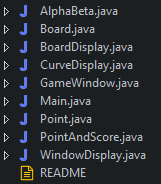
\includegraphics[width=0.40\textwidth]{./ARBORESCENCE}~\\
\end{center}
\end{figure}
\newpage


Ainsi que les différentes méthodes de notre class Board
\begin{figure}[!ht]
\begin{center}
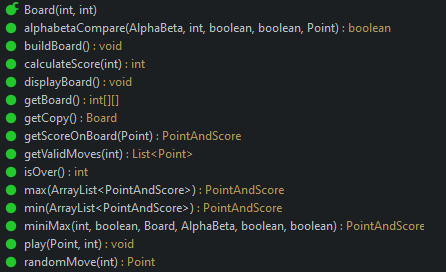
\includegraphics[width=0.65\textwidth]{./METHODESBOARD}
\end{center}
\end{figure}
\\
Et voici comment se présente le déroulement de la partie dans la console.
\begin{figure}[!ht]
\begin{center}
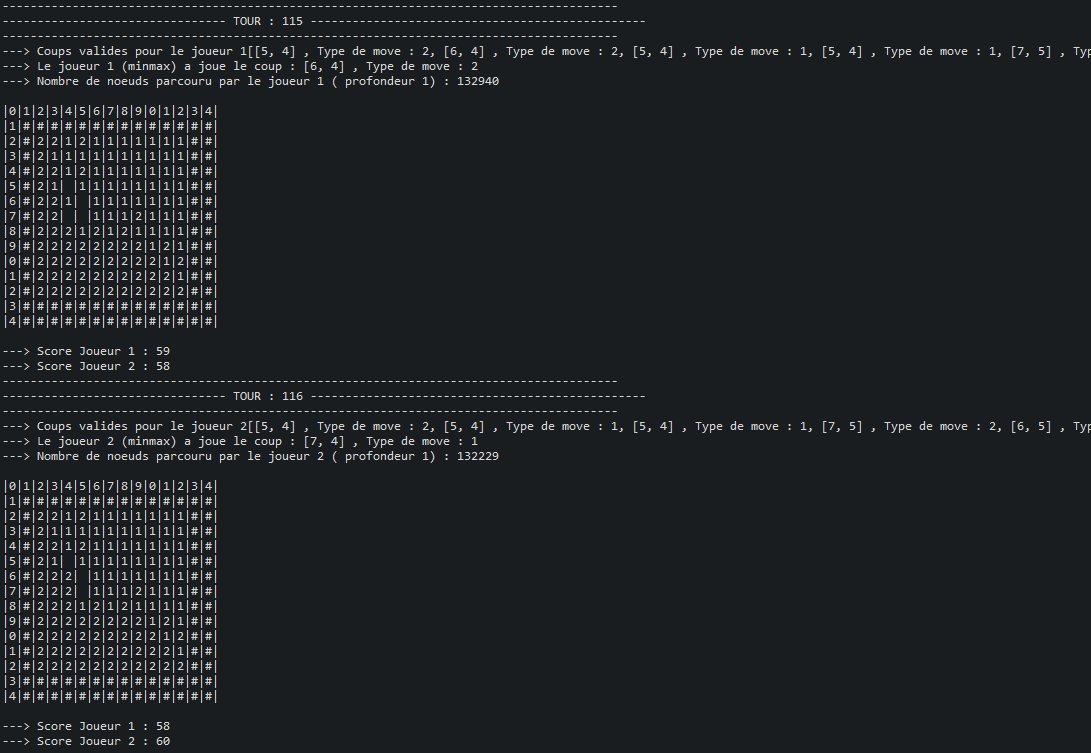
\includegraphics[width=0.95\textwidth]{./INTROJEU}
\end{center}
\end{figure}



